\section{Head to head}

\subsection{Network structure}

\cref{tab:results-head-to-head-accuracy} shows the \gls{rps} values and accuracy of the head to head network. In the evaluation data set, 38.1\% of all matches ended in a home victory.
\begin{table}
    \centering
    \begin{tabulary}{\textwidth}{| L | L || L | L | L || L |}
        \hline
        \multicolumn{2}{| l ||}{\textbf{Hidden layer}}  & \multicolumn{3}{l ||}{\textbf{\gls{rps} values}} & \\\hline
        \textbf{Activation} & \textbf{Size}             & \textbf{Min}  & \textbf{Max}  & \textbf{Mean} & \textbf{Accuracy} \\\hline
        \gls{relu}          & 16                        & 0.127         & 0.479         & 0.300         & 0.387 \\\hline
        \gls{relu}          & 32                        & 0.0733        & 0.571         & 0.234         & 0.391 \\\hline
        \gls{relu}          & 64                        & 0.0889        & 0.548         & 0.232         & 0.397 \\\hline
        \gls{relu}          & 128                       & 0.0692        & 0.586         & 0.238         & 0.387 \\\hline
        
        \hline
        
        Sigmoid             & 16                        & 0.0823        & 0.553         & 0.236         & 0.394 \\\hline
        \rowcolor{correct}
        Sigmoid             & 32                        & 0.111         & 0.468         & 0.228         & 0.401 \\\hline
        Sigmoid             & 64                        & 0.081         & 0.557         & 0.232         & 0.381 \\\hline
        
        \hline
        
        \Gls{tanh}          & 16                        & 0.0904        & 0.537         & 0.232         & 0.397 \\\hline
        \Gls{tanh}          & 32                        & 0.0883        & 0.537         & 0.231         & 0.384 \\\hline
        \Gls{tanh}          & 64                        & 0.0959        & 0.523         & 0.230         & 0.384 \\\hline
    \end{tabulary}
    \caption{Accuracy of the head to head network, with different hidden layer configurations. The row colored green shows the configuration with most promising results.}
    \label{tab:results-head-to-head-accuracy} 
\end{table}

Using a hidden layer with 32 nodes activated by the sigmoid function yielded the most promising results, and will therefore be used when evaluating the profitability of the network. \cref{tab:results-head-to-head-accuracy-2016-2017} shows the \gls{rps} values and prediction accuracy when evaluating the same configuration over the 2016-2017 season. Unfortunately, the network did not perform better than the benchmark model for any of the seasons.
\begin{table}
    \centering
    \begin{tabulary}{\textwidth}{| L | L | L || L |}
        \hline
        \multicolumn{3}{| l ||}{\textbf{\gls{rps} values}}  &                   \\\hline
        \textbf{Min}    & \textbf{Max}  & \textbf{Mean}     & \textbf{Accuracy} \\\hline
        0.0933          & 0.727         & 0.220             & 0.497             \\\hline
    \end{tabulary}
    \caption{Prediction accuracy of the head to head network for the 2016-2017 season of the English Premier League, using the most promising hidden layer configuration.}
    \label{tab:results-head-to-head-accuracy-2016-2017} 
\end{table}


\subsection{Betting results}

\subsubsection{English Premier League 2015-2016}

\cref{fig:results-head-to-head-2015-2016-fixed-bet,fig:results-head-to-head-2015-2016-fixed-return,fig:results-head-to-head-2015-2016-kelly-ratio,fig:results-head-to-head-2015-2016-variance-adjusted} show the development of the \gls{roi} generated by the head to head network over the English Premier League season 2015-2016.
\begin{figure}
    \centering
    \includegraphics[width=\textwidth]{results/head-to-head/2015-2016/fixed-bet-10.png}
    \caption{\gls{roi} over the span of the English Premier League season 2015-2016 using the head to head network and the fixed bet strategy.}
    \label{fig:results-head-to-head-2015-2016-fixed-bet}
\end{figure}
\begin{figure}
    \centering
    \includegraphics[width=\textwidth]{results/head-to-head/2015-2016/fixed-return-10.png}
    \caption{\gls{roi} over the span of the English Premier League season 2015-2016 using the head to head network and the fixed return strategy.}
    \label{fig:results-head-to-head-2015-2016-fixed-return}
\end{figure}
\begin{figure}
    \centering
    \includegraphics[width=\textwidth]{results/head-to-head/2015-2016/kelly-ratio-10.png}
    \caption{\gls{roi} over the span of the English Premier League season 2015-2016 using the head to head network and the Kelly ratio strategy.}
    \label{fig:results-head-to-head-2015-2016-kelly-ratio}
\end{figure}
\begin{figure}
    \centering
    \includegraphics[width=\textwidth]{results/head-to-head/2015-2016/variance-adjusted-10.png}
    \caption{\gls{roi} over the span of the English Premier League season 2015-2016 using the head to head network and the variance adjusted strategy.}
    \label{fig:results-head-to-head-2015-2016-variance-adjusted}
\end{figure}

\cref{tab:fig:results-head-to-head-2015-2016-roi} shows a summary of the \gls{roi} values achieved by the different strategies when used by the head to head network. The table shows the final \gls{roi} for the least profitable and most profitable simulations, together with the average final \gls{roi}.
\begin{table}
    \centering
    \begin{tabulary}{\textwidth}{| L || L | L | L |}
        \hline
                            & \multicolumn{3}{l |}{\textbf{Final \gls{roi}}} \\\hline
        \textbf{Strategy}   & \textbf{Min}  & \textbf{Max}  & \textbf{Mean} \\\hline
        Fixed bet           & 0.16          & 0.61          & 0.40 \\\hline
        Fixed return        & -0.053        & 0.092         & 0.025 \\\hline
        Kelly ratio         & 0.44          & 3.1           & \cellcolor{correct} 2.0 \\\hline
        Variance adjusted   & -0.070        & 0.057         & -0.0080 \\\hline
    \end{tabulary}
    \caption{Final \gls{roi} values for the four strategies when using the head to head network during the 2015-2016 season of the English Premier League. The green colored cell was the most profitable strategy (on average).}
    \label{tab:fig:results-head-to-head-2015-2016-roi}
\end{table}
  
\cref{fig:results-head-to-head-2015-2016-odds-prob} shows the bets placed during the 2015-2016 season of the English Premier League. The probabilities are generated by a random instance of the head to head network.
\begin{figure}
    \centering
    \includegraphics[width=\textwidth]{results/head-to-head/2015-2016/odds-prob.png}
    \caption{Offered odds and predicted probabilities for the bets placed during the 2015-2016 season of the English Premier League. The probabilities are generated by the head to head network.}
    \label{fig:results-head-to-head-2015-2016-odds-prob}
\end{figure}
      

\subsubsection{English Premier League 2016-2017}

\cref{fig:results-head-to-head-2016-2017-fixed-bet,fig:results-head-to-head-2016-2017-fixed-return,fig:results-head-to-head-2016-2017-kelly-ratio,fig:results-head-to-head-2016-2017-variance-adjusted} show the development of the \gls{roi} generated by the head to head network over the English Premier League season 2016-2017.
\begin{figure}
    \centering
    \includegraphics[width=\textwidth]{results/head-to-head/2016-2017/fixed-bet-10.png}
    \caption{\gls{roi} over the span of the English Premier League season 2016-2017 using the head to head network and the fixed bet strategy.}
    \label{fig:results-head-to-head-2016-2017-fixed-bet}
\end{figure}
\begin{figure}
    \centering
    \includegraphics[width=\textwidth]{results/head-to-head/2016-2017/fixed-return-10.png}
    \caption{\gls{roi} over the span of the English Premier League season 2016-2017 using the head to head network and the fixed return strategy.}
    \label{fig:results-head-to-head-2016-2017-fixed-return}
\end{figure}
\begin{figure}
    \centering
    \includegraphics[width=\textwidth]{results/head-to-head/2016-2017/kelly-ratio-10.png}
    \caption{\gls{roi} over the span of the English Premier League season 2016-2017 using the head to head network and the Kelly ratio strategy.}
    \label{fig:results-head-to-head-2016-2017-kelly-ratio}
\end{figure}
\begin{figure}
    \centering
    \includegraphics[width=\textwidth]{results/head-to-head/2016-2017/variance-adjusted-10.png}
    \caption{\gls{roi} over the span of the English Premier League season 2016-2017 using the head to head network and the variance adjusted strategy.}
    \label{fig:results-head-to-head-2016-2017-variance-adjusted}
\end{figure}

\cref{tab:fig:results-head-to-head-2016-2017-roi} shows a summary of the \gls{roi} values achieved by the different strategies when used by the head to head network. The table shows the final \gls{roi} for the least profitable and most profitable simulations, together with the average final \gls{roi}.
\begin{table}
    \centering
    \begin{tabulary}{\textwidth}{| L || L | L | L |}
        \hline
                            & \multicolumn{3}{l |}{\textbf{Final \gls{roi}}} \\\hline
        \textbf{Strategy}   & \textbf{Min}  & \textbf{Max}  & \textbf{Mean} \\\hline
        Fixed bet           & -0.25         & -0.12         & -0.20 \\\hline
        Fixed return        & -0.038        & 0.07          & -0.018 \\\hline
        Kelly ratio         & -1.0          & -1.0          & -1.0 \\\hline
        Variance adjusted   & -0.024        & 0.014         & \cellcolor{correct} -0.0060 \\\hline
    \end{tabulary}
    \caption{Final \gls{roi} values for the four strategies when using the head to head network during the 2016-2017 season of the English Premier League. The green colored cell was the most profitable strategy (on average).}
    \label{tab:fig:results-head-to-head-2016-2017-roi}
\end{table}

\cref{fig:results-head-to-head-2016-2017-odds-prob} shows the bets placed during the 2016-2017 season of the English Premier League. The probabilities are generated by a random instance of the head to head network.
\begin{figure}
    \centering
    \includegraphics[width=\textwidth]{results/head-to-head/2016-2017/odds-prob.png}
    \caption{Offered odds and predicted probabilities for the bets placed during the 2016-2017 season of the English Premier League. The probabilities are generated by the head to head network.}
    \label{fig:results-head-to-head-2016-2017-odds-prob}
\end{figure}


\subsubsection{Summary}

The network did not achieve consistent good results. The first season, the fixed bet and Kelly ratio strategies performed well, gaining profits for all instances. The second season, however, the same strategies achieved \glspl{roi} of -0.25 and -1.0, respectively.

\cref{fig:results-head-to-head-2015-2016-odds-prob,fig:results-head-to-head-2016-2017-odds-prob} show the connection between odds and probabilities predicted by the head to head network. The head to head network struggles with sparse predictions. This is likely due to how rapidly teams change in football. Between each season, and in January, teams have the opportunity to buy and sell players. A team being relegated from the English Premier League might be forced to sell their best players, reducing their strengths. Other teams receive a lot of money from their owners, making them able to improve their squad greatly between two seasons. This makes it difficult to predict the results of a match based on the previous meetings between the two teams. The training procedure therefore approximates the outcome distribution in the training data set. Over the two seasons, the prediction models won approximately 19.2\% of all bets placed, with an average odds of 4.89.